\documentclass[a4paper]{article}

%% Language and font encodings
\usepackage[english]{babel}
\usepackage[utf8]{inputenc}
\usepackage[T1]{fontenc}

%% Sets page size and margins
\usepackage[a4paper,top=3cm,bottom=2cm,left=3cm,right=3cm,marginparwidth=1.75cm]{geometry}

%% Useful packages
\usepackage[tbtags]{amsmath}
\usepackage{mathtools}
\usepackage{graphicx}
\usepackage[colorinlistoftodos]{todonotes}
\usepackage[colorlinks=true, allcolors=blue]{hyperref}
\usepackage{color}
\usepackage{tikz}
\usepackage{titlesec}
\usepackage{caption}
\usepackage[shortlabels]{enumitem}
\usepackage{setspace}
\usepackage{authblk}
\usepackage{floatrow}
\usepackage{blkarray, bigstrut}

\floatstyle{plaintop}
\restylefloat{table}

\usetikzlibrary{shapes.geometric, arrows}

% package to manage citations
\usepackage[backend=bibtex,style=authoryear-comp,sorting=nyt,isbn=false,url=false, natbib=true, doi=false]{biblatex}
\addbibresource{bibliography.bib}

\tikzstyle{startstop_big} = [rectangle, rounded corners, minimum width=3cm, minimum height=1cm,text centered, draw=black,text width = 8.5cm, fill=red!30]
\tikzstyle{startstop} = [rectangle, rounded corners, minimum width=3cm, minimum height=1cm,text centered, draw=black,text width = 5cm, fill=red!30]
\tikzstyle{io} = [trapezium, trapezium left angle=70, trapezium right angle=110, minimum width=2cm, minimum height=1cm, text centered, draw=black, fill=blue!30]
\tikzstyle{process} = [rectangle, minimum width=3cm, minimum height=1cm, text centered, text width = 3cm, draw=black, fill=orange!30]
\tikzstyle{process_wide_3pt5cm} = [rectangle, minimum width=3cm, minimum height=1cm, text centered, text width = 3.5cm, draw=black, fill=orange!30]
\tikzstyle{process_wide_4cm} = [rectangle, minimum width=3cm, minimum height=1cm, text centered, text width = 4cm, draw=black, fill=orange!30]
\tikzstyle{process_wide_4pt5cm} = [rectangle, minimum width=3cm, minimum height=1cm, text width = 4.5cm, draw=black, fill=orange!30]
\tikzstyle{process_wide_5cm} = [rectangle, minimum width=3cm, minimum height=1cm, text width = 5cm, draw=black, fill=orange!30]
\tikzstyle{decision} = [diamond, minimum width=1cm, minimum height=1cm,text centered,text width = 2.25cm, draw=black, fill=green!30]
\tikzstyle{arrow} = [thick,->,>=stealth]

\definecolor{ErasmusBlue}{RGB}{12, 32, 116}

%Use 4 levels of sections using package titlesec
%\setcounter{secnumdepth}{4}
\newcommand{\subsubsubsection}[1]{\paragraph{#1}\mbox{}\\\\}
\newcommand*\diff{\mathop{}\!\mathrm{d}}
%\newcommand{\argmax}[1]{\underset{#1}{\operatorname{arg}\,\operatorname{max}}\;}
\DeclareMathOperator{\argmax}{arg\,max}
\DeclarePairedDelimiter\abs{\lvert}{\rvert}%
\DeclarePairedDelimiter\norm{\lVert}{\rVert}%

\let\bmath\boldsymbol
\let\rmn\mathrm
\newcommand{\Hline}
{
\hline
\hline
}

\renewcommand{\thesection}{Appendix \Alph{section}}

\begin{document}
\title{\LARGE \textbf{Supplementary Material for ``A Personalized Screening Strategy to Monitor the Development of Chronic Allograft Failure in Renal Rransplant Recipients''}}

\author[1,2,*]{\large Hessel Peters-Sengers}
\author[3,*]{Anirudh Tomer}
\author[4]{Sandrine Florquin}
\author[5,6]{Ewout W. Steyerberg}
\author[1]{Frederike J. Bemelman}
\author[3,\$]{Dimitris Rizopoulos}
\author[4,7,\$]{Jesper Kers}
\affil[1]{\footnotesize Division of Internal Medicine, Renal Transplant Unit, Academic Medical Center, Amsterdam, The Netherlands}
\affil[2]{Center for Experimental and Molecular Medicine (CEMM), Academic Medical Center, Amsterdam, The Netherlands}
\affil[3]{Department of Biostatistics, Erasmus University Medical Center, Rotterdam, The Netherlands}
\affil[4]{Department of Pathology, Academic Medical Center, Amsterdam, The Netherlands}
\affil[5]{Department of Public Health, Erasmus University Medical Center, Rotterdam, The Netherlands}
\affil[6]{Department of Medical Statistics and Bioinformatics, Leiden University Medical Center, Leiden, The Netherlands}
\affil[7]{Van 't Hoff Institute for Molecular Sciences (HIMS), University of Amsterdam, Amsterdam, The Netherlands}
\affil[*,\$]{Authors contributed equally to the study}

\date{}

\maketitle

\input{mainmatter/jm_framework}
\clearpage
% !TEX root =  ../appendix.tex

\section{Joint Model for the Kidney Transplant Dataset}
\label{sec : jm_amctx}
A total of 239 kidney transplant patients were included in the data set. The transplantation characteristics of these patients is presented in Table \ref{tab : baseline_characteristics}. The data set also includes periodical measurements of SCr and PCR. Our goal is to check if SCr and PCR both, are useful to predict graft failure. To this end, we model the two longitudinal outcomes and graft failure together using the joint modeling framework described in \ref{sec : jm_amctx}. In this model we use log transformed values of both SCr and PCR \citep{fournier2016joint}. More specifically, we model the impact of log(SCr) value and log(SCr) velocity, log(PCR) value and log(PCR) velocity, and transplantation characteristics on the hazard of graft failure. In this regard, the JM consists of a multivariate longitudinal sub-model to model the evolution of SCr and PCR and a relative risk sub-model to model the impact of transplantation characteristics and biomarkers on the hazard of graft failure. The longitudinal evolution of the two outcomes over time is modeled flexibly using B-splines. The model formulation for PCR outcome is as follows (for SCr outcome it is same):
\begin{equation}
\label{eq : long_model_prias}
\begin{aligned}
\log \mbox{PCR}(t) &= \beta_0 + \beta_1 \mbox{rec\_age} + \beta_2 \mbox{d\_age} + \beta_3 \mbox{d\_bmi} + \beta_4 \mbox{rec\_bmi} + \beta_5 \mbox{cit}\\
&+ \beta_6 \mbox{hla} + \beta_7 \mbox{pra}+ \beta_8 \mbox{dial\_days} + \beta_9 \mbox{ah\_nr} + \beta_{10} \mbox{rec\_gender} + \beta_{11} \mbox{d\_gender} \\
&+ \beta_{12} \mbox{dgf} + \beta_{13} \mbox{prev\_tp} + \beta_{14} \mbox{dm} + \beta_{15} \mbox{hvdis}+ \beta_{16} \mbox{d\_cadaveric}\\
&+\sum_{k=1}^4 \beta_{k+16} B_k(t,\mathcal{K}) +  b_{i0} + \sum_{k=1}^4 b_{ik} B_k(t,\mathcal{K}) + 
\varepsilon_i(t),
\end{aligned}
\end{equation}
where $B_k(t, \mathcal{K})$ denotes the $k$-th basis function of a B-spline with three internal knots at $\mathcal{K} =\{0.082, 0.219, 1\}$ (30 and 80 days recommended by the clinicians) years, and boundary knots at 0.039 and 6 years (minimum and 0.95 quantile of the time of measurements two outcomes). The quantitative transplantation characteristics are standardized to avoid convergence issues in parameter estimation. For the relative risk sub-model the hazard function we fit is given by:
\begin{equation}
\label{eq : hazard_prias}
\begin{aligned}
h_i(t) &= h_0(t) \exp\big\{\gamma_1 \mbox{prev\_tp} + \gamma_2 \mbox{hla}  + \gamma_3 \mbox{cit} + \gamma_4 \mbox{dial\_days} \\
& + \alpha_{11} m_{i1}(t) + \alpha_{12} m'_{i1}(t) + \alpha_{21} m_{i2}(t) + \alpha_{22} m'_{i2}(t)\big\},
\end{aligned}
\end{equation}
where $\alpha_{11}, \alpha_{12}, \alpha_{21}$ and $\alpha_{22}$ are measures of strength of the association between hazard of graft failure and $\log \mbox{PCR}$ value $m_{i1}(t)$, $\log \mbox{PCR}$ velocity $m'_{i1}(t)$, $\log \mbox{SCr}$ value $m_{i1}(t)$ and $\log \mbox{SCr}$ velocity $m'_{i2}(t)$ respectively.

The parameters of the JM are estimated using the R package \textbf{JMbayes} \citep{rizopoulosJMbayes}, which uses the Bayesian methodology to estimate the model parameters. The parameter estimates for the relative risk sub-model are provided in Table \ref{tab : relative_risk}. Since the quantitative variables are standardized, the effect sizes correspond to one standard deviation increase in the corresponding variable.  The parameter estimates for the longitudinal sub-model for SCr and PCR are provided in Table \ref{tab : creatinine_long} and Table \ref{tab : pcr_long}, respectively. To avoid the tricky interpretation of variables corresponding to evolution over time, instead the evolution of SCr and PCR over time is depicted in Figure \ref{fig : creatinine_evolution}, and Figure \ref{fig : pcr_evolution}, respectively.

\begin{table}[!htb]
\begin{center}
\caption{Observed transplantation characteristics of the studied population (n = 239).}
\label{tab : baseline_characteristics}
\begin{tabular}{llr}
\Hline
\multicolumn{3}{c}{Quantitative characteristics} \\
\hline
Name & Abbreviation & Mean (SD) \\ 
\hline
Receiver age (at baseline) & rec\_age & 50.70 (13.09) \\
Donor age & d\_age & 49.73 (12.66) \\
Donor BMI & d\_bmi & 25.10 (4.43) \\
Receiver BMI & rec\_bmi & 25.43 (4.31) \\
Cold ischemia time (minutes) & cit & 887.25 (522.95)\\
\#HLA A, B and DR mismatches & hla & 2.81 (1.57)\\
Panel reactive antibody (\%) & pra & 4.81 (14.20) \\
\#Days on dialysis before transplant & dial\_days & 1334.91 (1283.93)\\
\#Anti-hypertensive medicaments & ah\_nr & 1.58 (0.96)\\
\hline
\\
\multicolumn{3}{c}{Categorical characteristics}\\
\hline
Name & Abbreviation & Category (\%) \\
\hline
Receiver gender & rec\_gender & Female (42.68 \%)\\
Donor gender & d\_gender & Female (56.49 \%)\\
Delayed graft function after transplant & dgf & No (67.78 \%)\\
Previous transplantation & prev\_tp & No (84.45 \%)\\
Diabetes mellitus & dm & No (84.52 \%)\\
Known cardiovascular events before transplant & hvdis & No (61.92 \%)\\
Deceased donor & d\_cadaveric & No (25.94 \%)\\
\hline     
\end{tabular}
\end{center}
\end{table}

\begin{table}[!htb]
\begin{center}
\caption{Relative risk sub-model estimates for mean and 95\% credible interval.}
\label{tab : relative_risk}
\begin{tabular}{lrrrrr}
\Hline
Variable               & Mean   & Std. Dev & 2.5\%  & 97.5\% & P              \\
\hline
Previous transplant: Yes      & 0.305  & 0.339    & -0.099 & 0.986  & 0.352          \\
\#HLA mismatches between donor and recipient                & 0.048  & 0.093    & -0.114 & 0.269  & 0.620          \\
Cold ischemia time                & -0.051 & 0.105    & -0.277 & 0.133  & 0.644          \\
\#Days on dialysis before transplant         & -0.013 & 0.102    & -0.251 & 0.178  & 0.934          \\
$\log \mbox{PCR}$        & 0.145  & 0.125    & -0.056 & 0.431  & 0.188          \\
Slope($\log \mbox{PCR}$)        & 0.021  & 0.058    & -0.076 & 0.145  & 0.828          \\
$\log \mbox{SCr}$ & 1.599  & 0.241    & 1.067  & 2.063  & \textless0.000 \\
Slope($\log \mbox{SCr}$)  & 0.203  & 0.123    & -0.017 & 0.443  & 0.082  \\
\hline
\end{tabular}
\end{center}
\end{table}

\begin{table}[!htb]
\begin{center}
\caption{Parameter estimates for the longitudinal sub-model for SCr.}
\label{tab : creatinine_long}
\begin{tabular}{lrrrrr}
\Hline
Variable                                                                         & Mean   & Std. Dev & 2.5\%  & 97.5\% & P              \\
\hline
Intercept                                                                      & 5.226  & 0.080    & 5.064  & 5.378  & \textless0.000 \\
Receiver age                                                                   & -0.063 & 0.022    & -0.107 & -0.019 & 0.010          \\
Donor age                                                                          & 0.083  & 0.020    & 0.045  & 0.119  & \textless0.000 \\
Donor BMI                                                                          & -0.011 & 0.021    & -0.054 & 0.028  & 0.612          \\
Receiver BMI                                                                         & 0.018  & 0.023    & -0.025 & 0.060  & 0.420          \\
\#HLA mismatches between donor and recipient                                                                         & 0.020  & 0.022    & -0.022 & 0.065  & 0.342          \\
Panel reactive antibody percentage                                                                          & 0.048  & 0.027    & -0.008 & 0.100  & 0.082          \\
\#Anti-hypertensive medicaments                                                                           & 0.040  & 0.020    & 0.001  & 0.080  & 0.048          \\
Cold ischemia time                                                                         & 0.029  & 0.035    & -0.039 & 0.102  & 0.390          \\
\#Days on dialysis before transplant                                                                   & 0.015  & 0.029    & -0.042 & 0.071  & 0.580          \\
Receiver gender: Male                                                                     & 0.197  & 0.042    & 0.111  & 0.276  & \textless0.000 \\
Previous transplant: Yes                                                                & 0.016  & 0.064    & -0.115 & 0.141  & 0.786          \\
Donor gender: Male                                                                      & 0.053  & 0.042    & -0.027 & 0.136  & 0.198          \\
Delayed graft function: Yes                                                                       & 0.118  & 0.049    & 0.025  & 0.216  & 0.006          \\
Diabetes Mellitus: Yes                                                                        & -0.103 & 0.059    & -0.217 & 0.012  & 0.076          \\
Cardiovascular events before transplantation: Yes                                                                     & -0.047 & 0.043    & -0.129 & 0.044  & 0.272          \\
Deceased donor: Yes                                                                 & 0.163  & 0.082    & 0.004  & 0.313  & 0.044          \\
Spline: visit time [0.039, 0.082] years & -0.440 & 0.041    & -0.517 & -0.358 & \textless0.000 \\
Spline: visit time [0.082, 0.219] years & -0.182 & 0.053    & -0.284 & -0.081 & \textless0.000 \\
Spline: visit time [0.219, 1] years & -0.545 & 0.081    & -0.712 & -0.395 & \textless0.000 \\
Spline: visit time [1, 6] years & 0.007  & 0.083    & -0.155 & 0.176  & 0.946          \\
$\sigma$                                                                            & 0.190  & 0.001    & 0.187  & 0.192  & \\
\hline
\end{tabular}
\end{center}
\end{table}

\begin{table}[!htb]
\begin{center}
\caption{Parameter estimates for the longitudinal sub-model for PCR.}
\label{tab : pcr_long}
\begin{tabular}{lrrrrr}
\Hline
              Variable                                                                   & Mean   & Std. Dev & 2.5\%  & 97.5\% & P              \\
              \hline
Intercept                                                                      & 3.731  & 0.179    & 3.398  & 4.083  & \textless0.000 \\
Receiver age                                                                   & 0.030  & 0.052    & -0.066 & 0.138  & 0.604          \\
Donor age                                                                          & 0.209  & 0.047    & 0.118  & 0.301  & \textless0.000 \\
Donor BMI                                                                          & -0.019 & 0.051    & -0.121 & 0.084  & 0.716          \\
Receiver BMI                                                                         & -0.116 & 0.050    & -0.219 & -0.021 & 0.014          \\
\#HLA mismatches between donor and recipient                                                                         & -0.013 & 0.049    & -0.112 & 0.086  & 0.776          \\
Panel reactive antibody percentage                                                                          & 0.047  & 0.061    & -0.066 & 0.166  & 0.446          \\
\#Anti-hypertensive medicaments                                                                           & 0.056  & 0.047    & -0.03  & 0.147  & 0.208          \\
Cold ischemia time                                                                         & 0.062  & 0.082    & -0.097 & 0.211  & 0.468          \\
\#Days on dialysis before transplant                                                                   & 0.006  & 0.066    & -0.120 & 0.134  & 0.952          \\
Receiver gender: Male                                                                     & -0.026 & 0.094    & -0.207 & 0.166  & 0.798          \\
Previous transplant: Yes                                                                & 0.035  & 0.149    & -0.241 & 0.332  & 0.816          \\
Donor gender: Male                                                                      & 0.114  & 0.096    & -0.079 & 0.303  & 0.228          \\
Delayed graft function: Yes                                                                       & 0.043  & 0.118    & -0.174 & 0.275  & 0.740          \\
Diabetes Mellitus: Yes                                                                        & 0.153  & 0.135    & -0.124 & 0.396  & 0.256          \\
Cardiovascular events before transplantation: Yes                                                                     & -0.016 & 0.106    & -0.221 & 0.199  & 0.890          \\
Deceased donor: Yes                                                                  & 0.144  & 0.193    & -0.246 & 0.509  & 0.462          \\
Spline: visit time [0.039, 0.082] years & -0.821 & 0.090    & -0.989 & -0.638 & \textless0.000 \\
Spline: visit time [0.082, 0.219] years & -0.578 & 0.131    & -0.838 & -0.304 & \textless0.000 \\
Spline: visit time [0.219, 1] years & -0.898 & 0.160    & -1.218 & -0.587 & \textless0.000 \\
Spline: visit time [1, 6] years & 0.460  & 0.234    & 0.015  & 0.927  & 0.036          \\
$\sigma$                                                                            & 0.479  & 0.004    & 0.472  & 0.486  & \\
\hline
\end{tabular}
\end{center}
\end{table}

\begin{figure}[!htb]
\centerline{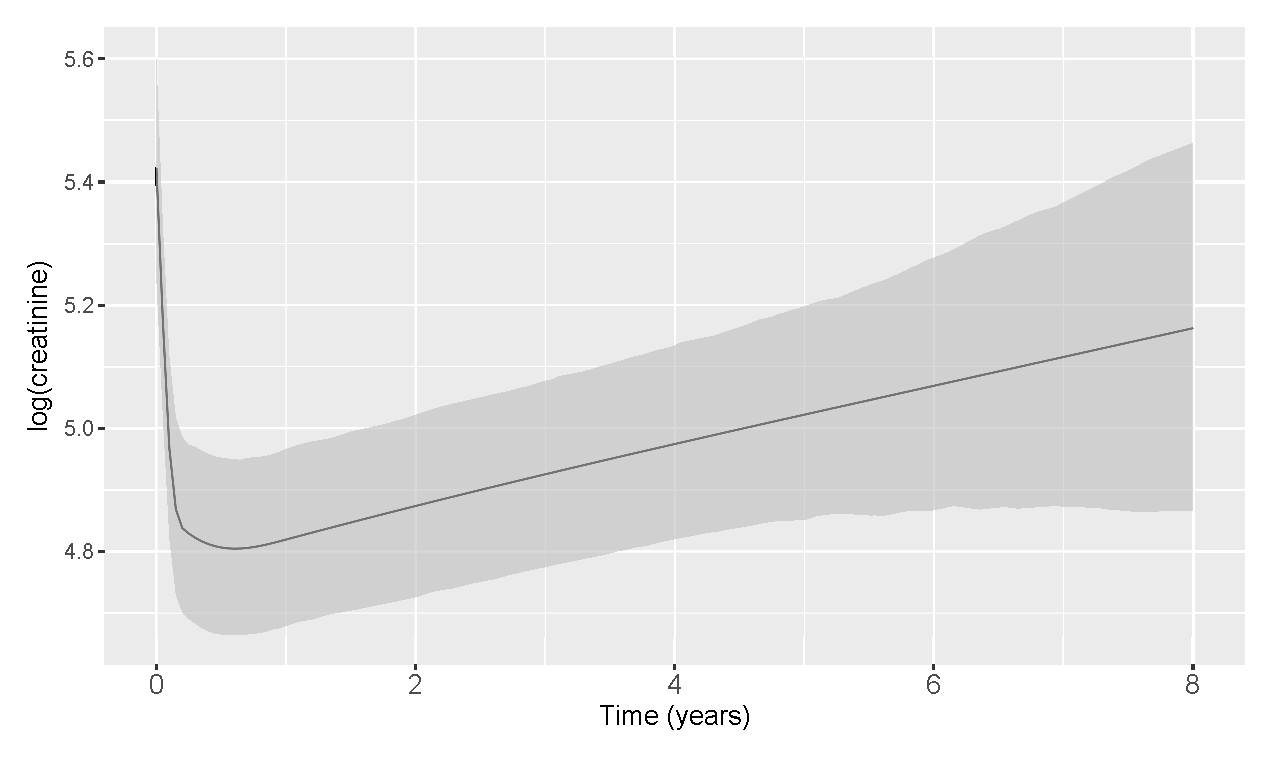
\includegraphics[width=\columnwidth]{images/creatinine.eps}}
\caption{Fitted longitudinal evolution of SCr and 95\% credible interval for a patient with the  transplantation characteristics described in Table \ref{tab : baseline_characteristics}.}
\label{fig : creatinine_evolution}
\end{figure}

\begin{figure}[!htb]
\centerline{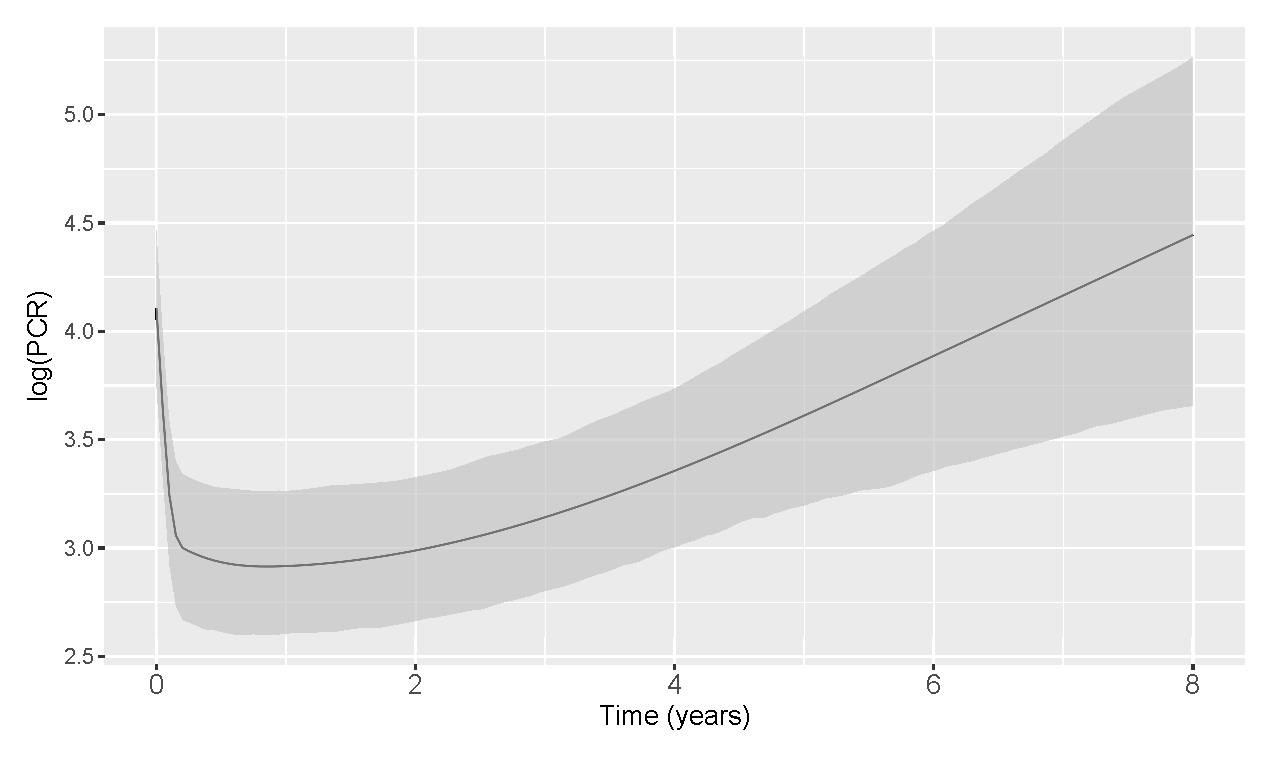
\includegraphics[width=\columnwidth]{images/pcr.eps}}
\caption{Fitted longitudinal evolution of PCR and 95\% credible interval for a patient with the  transplantation characteristics described in Table \ref{tab : baseline_characteristics}.}
\label{fig : pcr_evolution}
\end{figure}
\clearpage
% !TEX root =  ../ms.tex

\section{Personalized Schedules for Measurement of SCr}
\label{sec: simulation_study}
Currently, the schedule for measurement of SCr levels and fixed and common for all patients. SCr levels are measured 20 times in the first year after transplantation and every three months thereafter. Such fixed and frequent schedules are often burdensome for the patients. Patients who remain relatively stable after transplantation may not require frequent measurement of SCr in the first year. On the other hand, patients for whom the graft decays faster after the first year, a frequent schedule of SCr may be required to check the state of the graft. In this regard, instead of a common fixed schedule for all patients, we propose using a different schedule for every patient. More specifically, we propose using personalized schedules based on JMs \citet{drizopoulosPersScreening}. This is because, JMs utilize random effects and thus they are inherently patient specific. In this direction, firstly a full specification the joint distribution of SCr levels and time of graft failure is obtained. It is then used to define a patient-specific posterior predictive distribution of time of graft failure, given the observed SCr measurements. The optimal time of the next SCr measurement is the one at which the expected information gained from an extra SCr measurement is maximum. In order to create reasonable predictions, SCr measurements for the first 3 months are taken as per the fixed schedule. This time period corresponds to the time around which we observed an increase in the SCr profile.

Since the SCr measurements are already taken for the kidney transplant patients, in order to demonstrate the efficacy of the personalized schedules we conduct a small simulation. To this end, we first assume a population of kidney transplant patients, whose SCr and hazard of graft failure follow a JM of the form described in Section \ref{sec : joint_model}, with parameters equal to the posterior mean of parameters estimated from the joint model fitted to the kidney transplant dataset. From this population we sample 625 patients, which are further split into a training (575 patients) and test (50 patients) part. For the training patients we generate a graft failure time $T^*_i$ as well as a random and non-informative censoring time $C_i$. For the test patients the graft failure time $T^*_j$ and an intervention time $T^I_j$ is generated. The intervention time is the time at which the 6 month dynamic risk of graft failure of the patient becomes larger than a certain threshold $\kappa$. The choice of $\kappa$ dictates the amount of time at hand between intervention and graft failure. In this simulation we evaluate two $\kappa$ values, namely 0.05 and 0.025. 

Our goal is to compare personalized schedule with the currently used fixed schedule of SCr measurements. To this end, we first fit a joint model of the specification described in Section \ref{sec : joint_model} to the training data set and obtain a MCMC sample from the posterior distribution of the parameters of the JM. Using the fitted JM, we then iteratively schedule SCr measurements for the test patients, until the dynamic risk of graft failure \citep{rizopoulos2011dynamic} of the patients becomes larger than the threshold $\kappa$. Let $N^I_j$ denote the number of SCr measurements conducted for the $j$-th test patient. The time difference between the observed intervention time due to the schedule ($T^S_j$) and the true intervention time, that is, the intervention offset is denoted by $O^I_j = T^S_j - T^I_j$. Lastly, the failure offset $O^*_j = T^S_j - T^*j$ is the time at hand between the observed intervention time and the time of graft failure. Using the test patients, we calculate these measures for both personalized and fixed schedules. It is to be noted that in the ideal scenario, $N^I_j$ will be one, and offset $O^I_j$ will be zero. 

\begin{figure}[!htb]
\centerline{\includegraphics[width=\columnwidth]{images/nObspt05.eps}}
\caption{Boxplot of the number of SCr measurements $N^I_j$ for the test patients, for $\kappa = 0.05$.}
\label{fig : nObspt05}
\end{figure}

\begin{figure}[!htb]
\centerline{\includegraphics[width=\columnwidth]{images/truethrestimept05.eps}}
\caption{Boxplot of the intervention offset $O^I_j$ for the test patients, for $\kappa = 0.05$. The zero offset mark is displayed with the dashed line.}
\label{fig : truethrestimept05}
\end{figure}

\begin{figure}[!htb]
\centerline{\includegraphics[width=\columnwidth]{images/truestoptimept05.eps}}
\caption{Boxplot of the failure offset $O^*_j$ for the test patients, for $\kappa = 0.05$. The zero offset mark is displayed with the dashed line.}
\label{fig : truestoptimept05}
\end{figure}


A boxplot of the observed values of the number of SCr measurements $N^I_j$, intervention offset $O^I_j$ and failure offset $O^*_j$ are presented in Figure \ref{fig : nObspt05}, Figure \ref{fig : truethrestimept05} and Figure \ref{fig : truestoptimept05}, respectively. The mean number of SCr measurements for personalized schedule is 14.46 whereas it is 27.60 for fixed schedule. In addition the standard deviation for number of SCr measurements is 9.17 for fixed schedule and 4.03 for personalized schedule. That is, personalized schedule not only schedule less $N^I_j$ on average but the variation in $N^I_j$ from patient to patient is also less. The mean absolute intervention offset for personalized schedules is 0.445 whereas for fixed schedules it is 0.448. The personalized schedule also has less standard deviation for absolute $O^I_j$, with it being 0.285 for personalized schedule and being 0.338 for fixed schedule. There is indeed a risk that either of the schedule can exceed the true graft failure time. In this regard, 12\% of the times the graft failure is not detected for the test patients when fixed schedule is used. This rate is 14\% when personalized schedule is used. Furthermore, the mean absolute failure offset is 2.71 for personalized schedule and 2.76 for fixed schedule. The standard deviation for absolute $O^*_j$ is 1.97 for personalized schedule and 2.21 for fixed schedule. 

In order to reduce the risk of overshooting the true graft failure time we propose that a smaller $\kappa$ of 0.025 is used. The boxplot for the failure offset for this scenario is displayed in Figure \ref{fig : truestoptimept025}. In this scenario only for 6\% of the patients the graft failure time is exceeded. Boxplot for number of SCr measurements $N^I_j$ and intervention offset $O^I_j$ are displayed in Figure \ref{fig : nObspt025} and Figure \ref{fig : truethrestimept025}, respectively. However in this scenario, although the personalized schedule conducts less SCr measurements, it also exceeds the true intervention time more often than the fixed schedule.

\begin{figure}[!htb]
\centerline{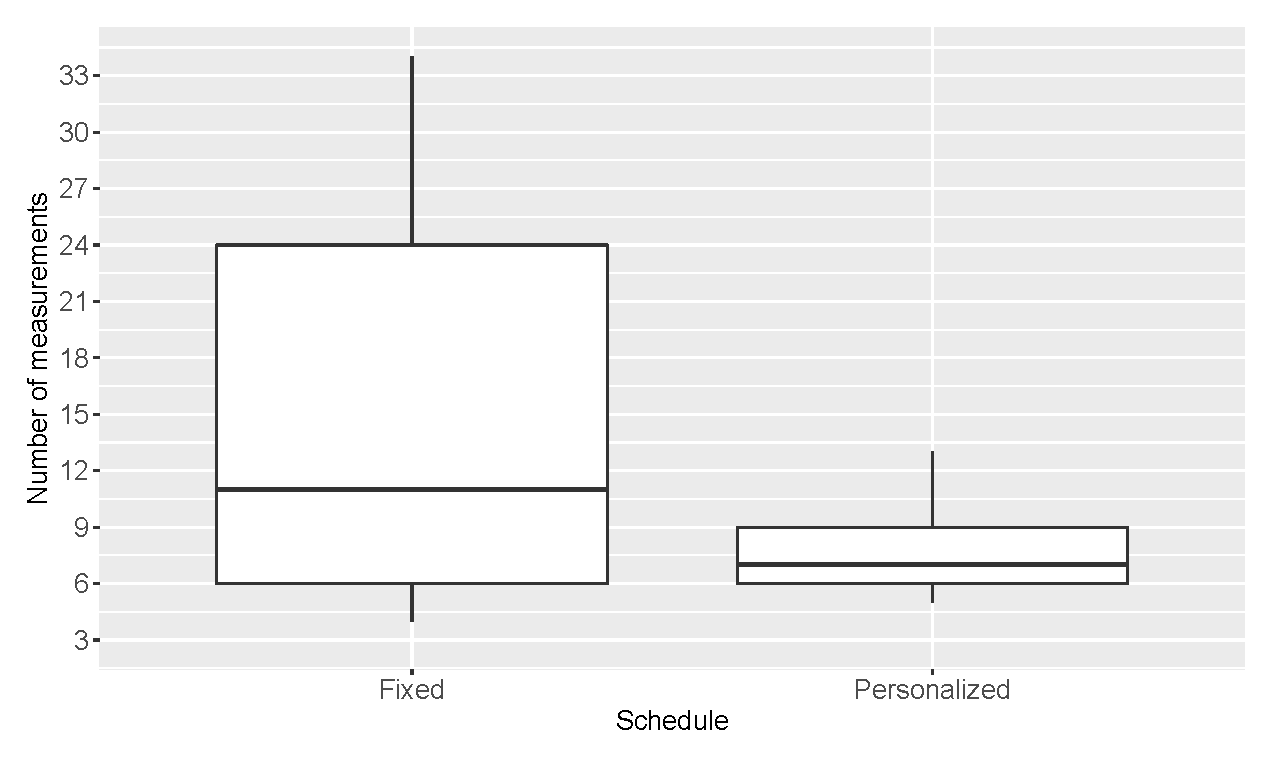
\includegraphics[width=\columnwidth]{images/nObspt025.eps}}
\caption{Boxplot of the number of SCr measurements $N^I_j$ for the test patients, for $\kappa = 0.025$.}
\label{fig : nObspt025}
\end{figure}

\begin{figure}[!htb]
\centerline{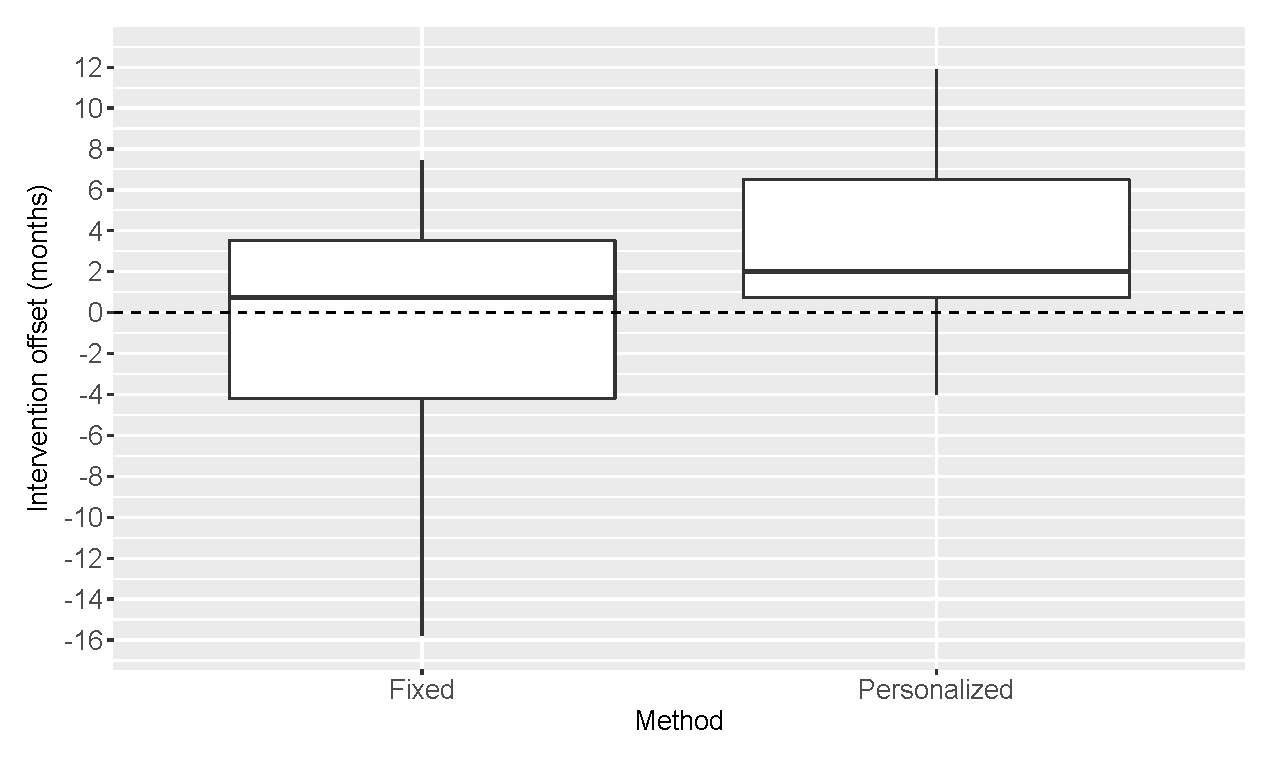
\includegraphics[width=\columnwidth]{images/truethrestimept025.eps}}
\caption{Boxplot of the intervention offset $O^I_j$ for the test patients, for $\kappa = 0.025$. The zero offset mark is displayed with the dashed line.}
\label{fig : truethrestimept025}
\end{figure}

\begin{figure}[!htb]
\centerline{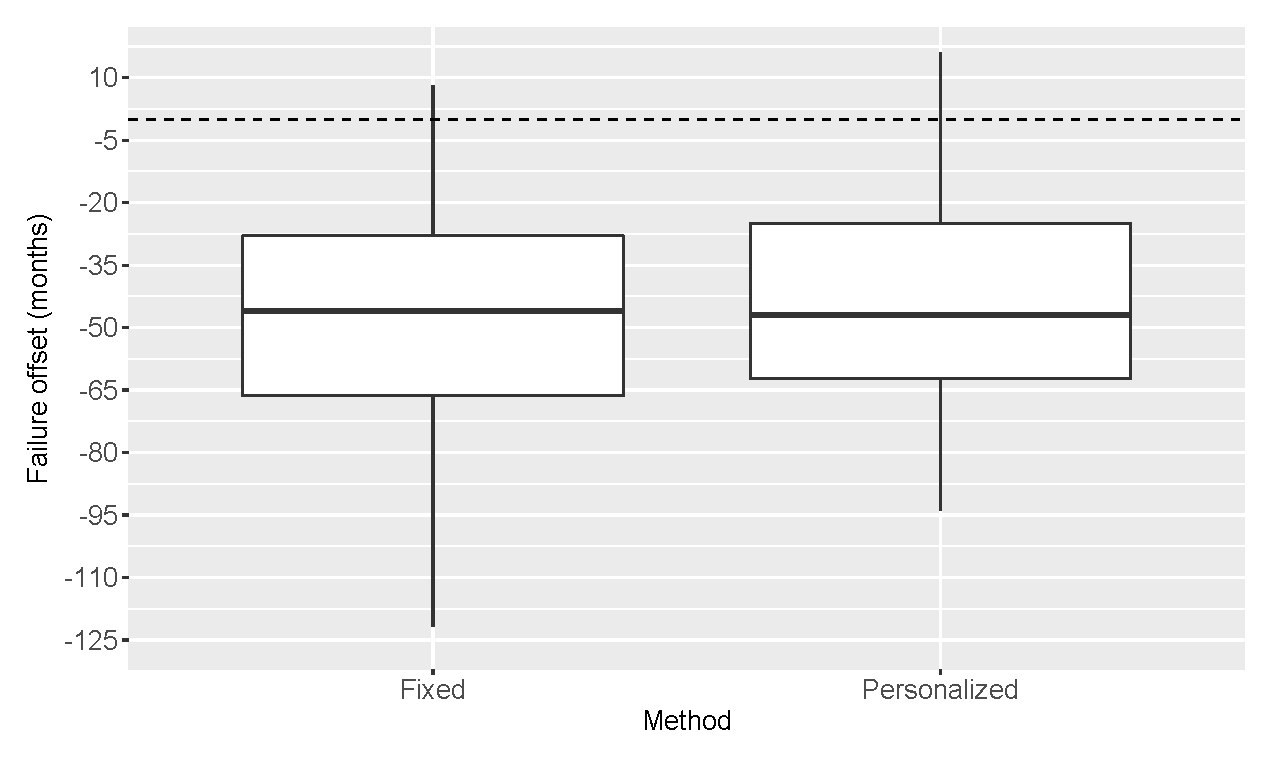
\includegraphics[width=\columnwidth]{images/truestoptimept025.eps}}
\caption{Boxplot of the failure offset $O^*_j$ for the test patients, for $\kappa = 0.025$. The zero offset mark is displayed with the dashed line.}
\label{fig : truestoptimept025}
\end{figure}
\clearpage
% !TEX root =  ../appendix.tex

\section{Source Code}
The source code for the joint model fitted to the kidney transplant data set can be found at:\\
\url{https://goo.gl/UefAW5}\\
The source code for the simulation study can be found at:\\
\url{https://goo.gl/jVVYeH}\\
A README file explaining the usage of the code can be found at:\\
\url{https://goo.gl/skFHNV}.\\



\clearpage
\printbibliography

\appendix

\end{document}